\documentclass[thesis.tex]{subfiles}

\begin{document}
\section{Definitions}
\todo[inline]{These will be defined elsewhere in the thesis, but are here so that this draft is understandable}
\begin{itemize}
\item
  Time is discrete: $1, \dots, T$.
\item
  We observe $n_a$ episodes of infection, indexed by $i$.
\item
  The $i$ in which episode $i$ occurs is tested at times
  $t_i = \{ t_{i,1}, \dots, t_{i,m_i} \}$.
\item
  Each observed episode has an unknown start of infection time $b_i$
  and end of infection time $e_i$ (the first and last day that the
  individual would test positive due to this episode respectively).
  These are realisations of the random variables $B_i$ and $E_i$
  respectively.
\item
  The duration of the infection is the number of days for which an
  individual tests positive, $D_i = E_i - B_i + 1$.
\item
  We assume that, for all episodes $i$, $D_i$ is iid and independent
  of the time of the infection. Define the survival function
  $\prob(D_i \geq t \mid B_i = b, \theta) = \prob(D_i \geq t \mid \theta) = S_\theta(t)$,
  where $\theta$ are the parameters controlling the survival
  distribution (the discussion in this document is valid regardless of
  the model specified for $S_\theta$ and hence we consider $\theta$
  as an arbitrary vector of parameters).
\item
  The beginning of episode $i$ is known to occur in the interval
  $[l_i^{(b)}, r_i^{(b)}]$, and similarly for the end of the infection
  in $[l_i^{(e)}, r_i^{(e)}]$.
\item
  $y_i(t)$ for $t \in t_i$ is a binary indicator giving the test
  result for individual $i$ at time $t$. Under the perfect testing
  assumption, $y_i(t) = 1$ if and only if $b_i \leq t \leq e_i$.
\item
  Throughout, the convention that lower-case letters are realisations of
  upper-case random variables is used.
\end{itemize}

\chapter{Estimating duration with infrequent testing} \label{perf-test}

The estimation of incidence from prevalence is sensitive to the tail of the duration distribution.
In \cref{E-ATACCC} I estimated the duration distribution from the ATACCC dataset, however, this study suffered from a small sample size and only 20 days of follow-up.
Therefore, the estimation of the tail of the duration distribution is driven by model assumptions.
This chapter develops methods to estimate the distribution using CIS data, which has less frequent sampling but a large sample size and long follow-up.

I take a Bayesian survival analysis approach to model the coarse sampling of the CIS (see \cref{perf-test:sec:problem}).
Flat priors can be unintentionally very informative, and hence (weakly) informative priors should be used.
Of particular interest is a strongly informative prior to combine the information in the CIS with the results of \cref{E-ATACCC} (see \cref{perf-test:sec:parameters-priors}).
Through a simulation study, I show that these methods perform well, and in this context are not sensitive to model or whether the prior is weakly or strongly informative (see \cref{perf-test:sec:simulation-study}).
However, application in reality must account for false negatives, the subject of \cref{E-imperf-test}.

\section{Problem description} \label{perf-test:sec:problem}

The CIS infrequently tests each individual, with tests occurring either weekly or monthly (see\todo{refer to section with CIS intro}).
The infrequent testing complicates analysis of the data in two ways: infection episodes can go undetected and the infection episode endpoints (start and end times) are known imprecisely.
This section explains these issues fully, and the remainder of the chapter develops a method to model them.

The first complication in the analysis is that infection episodes can be undetected, meaning no there are no positive tests associated with them.
This happens when an episode starts and ends between tests (see \cref{perf-test:fig:truncation}).
For these undetected episodes, there is no information on them episode, meaning that we do not even know how many of them occurred.
It is important to account for undetected episodes because they are systematically of shorter duration than detected episodes.
To see why this is the case, consider the undetected infection in the bottom of \cref{perf-test:fig:truncation}.
The infection episode depicted begins at time 33 and has a 10-day duration.
If the duration was 24 days (or longer), the individual would still have been detectable at their next test, and therefore would have been detected.
Undetected infections are a large problem in CIS because the interval between tests is often 28 days (see\todo{ref section on the survey design}), large relative to the duration of an infection episode.
\begin{figure}
  \centering 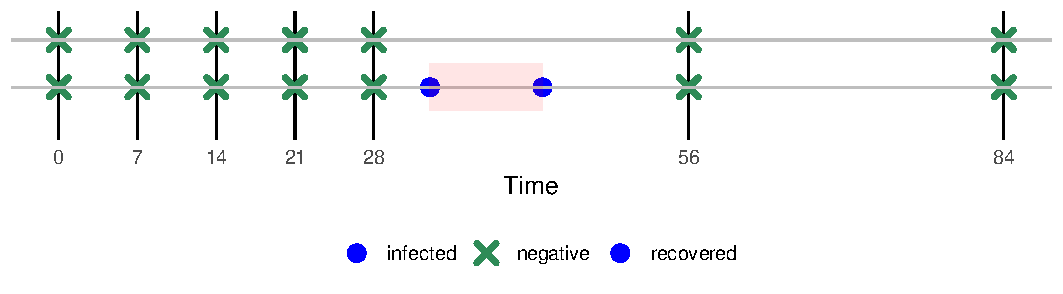
\includegraphics{cis-perfect-testing/truncation}
  \caption[Undetected episodes in CIS data]{An unknown number of infection episodes in CIS are undetected. Consider the two individuals shown here: we collect identical data for them (a series of negative tests) yet the top individual was never infected and the bottom individual was. See the main text for why this is an issue. \label{perf-test:fig:truncation}}
\end{figure}

The second complication is that the beginning and end times of detected infection episodes are known imprecisely.
The imprecision in the beginning of the infection episode arises because the only observation that an episode has started is that an individual was negative at one test, on day $l_i^{(b)}-1$ (the minus one is because the first day that the infection could have begun is the day after the negative test), and positive at the next test, on day $r_i^{(b)}$.
Similarly, the end of the infection episode is bounded by the final positive test on day $l_i^{(e)}$ and the following negative test on day $r_i^{(e)}+1$ (the plus one is because the last day that the infection could have ended is the day before the negative test).
\Cref{perf-test:fig:double-interval-censor} shows this issue graphically.
\begin{figure}
  \centering 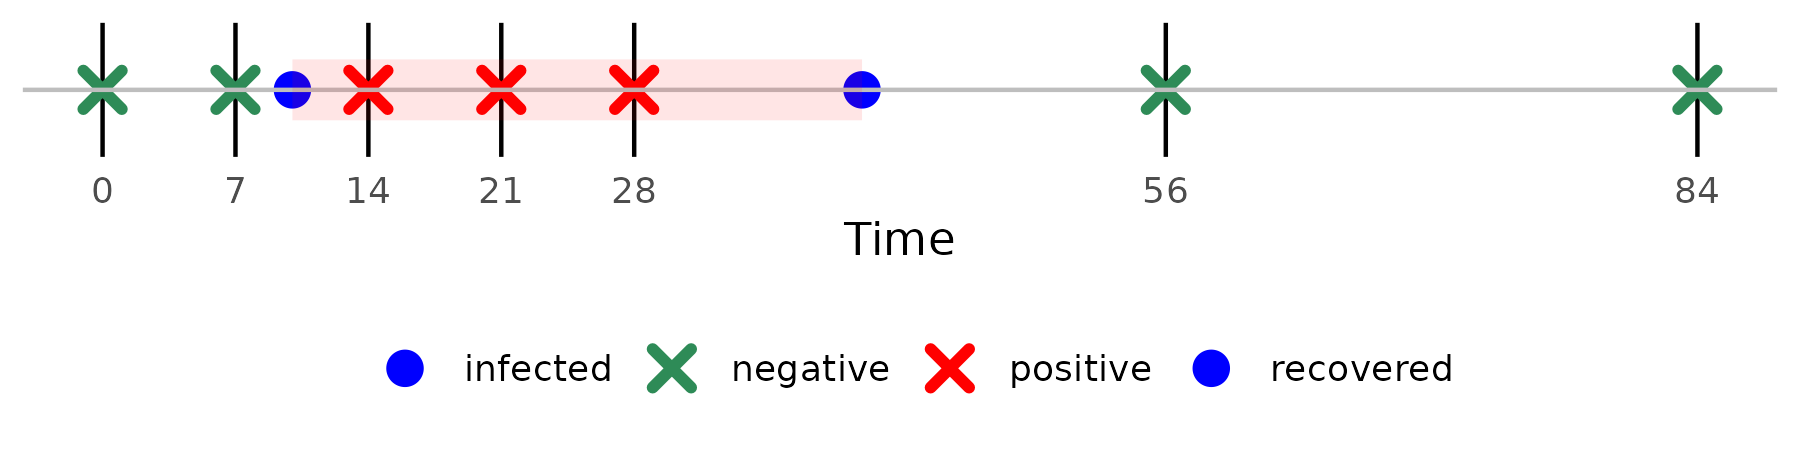
\includegraphics{cis-perfect-testing/double-interval-censor}
  \caption[Double-interval censoring in CIS data]{Episodes data in CIS is double interval censored, meaning that both the start and end of the episode are only known up to an interval. Demonstrated here by a participant who is recorded negative at time 7 to positive at time 14, bounding the start of the episode; similarly, changing from positive at time 28 to negative at time 56 bounds the end of the episode. \label{perf-test:fig:double-interval-censor}}
\end{figure}

I will base my analysis on the 4,800\todo{check number} of episodes that were first detected between 10th Oct 2020 and 6th Dec 2020 inclusive and have negatives bounding the start and end time of the episode.
That is, the individual in which the infection episode occurred tested negative at least once in the survey prior to the start of their infection episode, and they tested negative at least once after their infection episode ended.
Without a negative before the episode there is little information on the episode's length because it's start time could have occurred arbitrarily long ago.
The only episodes without a negative following the end of the episode are those in individuals lost to follow-up before their episode ended, which is extremely rare.
This filtering could bias the results of the study but will be considered in the same way as undetected episodes to avoid this.

In the remainder of this and the following chapter, I use survival analysis rather than the biomarker approach taken in \cref{E-ATACCC} for computational efficiency and data limitations arising from the study design.
In the biomarker approach, computational efficiency is an issue because the number of random effects scales with the number of detected infection episodes.
There are a large number of detected episodes in CIS; in the period I will consider, around 50 times more than in ATACCC.
Therefore, the biomarker approach would be computationally challenging with the large sample size in CIS.
The computational challenge is compounded by the data being stored in a TRE with the associated limited access to computational power and software.
The study design of CIS, with the infrequent sampling in the CIS study design, means that most detected episodes have only a single positive test.
Hence, there is no information on the viral load trajectory required to identify the random effects in the model used in \cref{E-ATACCC} or similar approaches.
While the biomarker approach does use more information per sample by taking into account the viral load as well as the binary test result (\ie whether the result is positive or negative), however, the available information is unlikely to be sufficient to overcome these problems.

\section{Survival analysis}

In survival analysis, the event at the start of the time of interest is the \emph{initiating event}, and the event at the end of the time of interest is the \emph{terminating event}.
It is broadly applicable to many domains, such as the time-to-failure for a mechanical system or the effect of a treatment on time spent in hospital.
In the context of this thesis, the distribution to estimate is the duration of positivity.
Therefore, the initiating event is when the duration starts; and the terminating event is when the duration ends.

Undetected events where we have information on missed events is unusual within the survival analysis literature.
Far more common is that there is no data on these events, a situation known as \emph{truncation}.
A situation that is particularly relevant is \emph{left truncation}, when only events lasting a minimum amount of time are observed.
A subtlety that makes the CIS different from standard left truncation is that information on individuals in which undetected infections occurred is available because they were enrolled in the study.
This information could be incorporated into the analysis, although doing so increases the computational burden and requires strong assumptions regarding reinfections without noticeably affecting the results (see \cref{appendix:total-model}).
In standard left truncation, nothing is known about the missed events.
As the information is not being incorporated here, standard left truncation methods remain applicable, and they can be modified to incorporate the additional information if desired.

When the time of the initiating and/or terminating events are not known exactly, the survival analysis literature refers to the event(s) as \emph{censored}.
Censored events are present in almost all survival analyses.
An event is \emph{left censored} if it is known to occur before a certain time, \emph{right censored} if it is known to occur after a certain time, and \emph{interval censored} if it is known to occur within an interval.
%Left and right censoring can be viewed as special cases of interval censoring where the lower bound is negative infinity or the upper bound is positive infinity respectively.
Interval censoring arises in CIS because we only observe the change from being not detectable (\ie: negative) at one test, to detectable (\ie: positive) at the following test and vice versa (see \cref{perf-test:fig:double-interval-censor}).
If both the initiating and terminating events are censored, then the event is \emph{doubly censored}.
Doubly censored data is more challenging to handle because the initiating event time and duration must be jointly modelled~\autocite[and references therein]{liSemiparametric}.
In CIS data both the initiating and the terminating events are interval censored.
Therefore, the CIS data is \emph{double interval censored}; approaches for double interval censoring are reviewed by \textcite{sunAnalysis,bogaertsSurvival}.

Few studies consider the combination of both double interval censoring and undetected or truncated events
This is especially true within the human biostatistical literature.
While this literature does contain theoretical frameworks which include the double censored and truncated case~\autocites{turnbullEmpirical}{dempsterMaximum}, they have been applied when the terminating event was either uncensored or right censored~\autocite{sunEmpirical,bacchettiNonparametric}.
The approach of these studies \autocite[and elsewhere, e.g.:][]{shenNonparametric} was to take a conditional likelihood approach, conditioning on both the truncation (a selection effect) and the period in which the initiating event is known to occur.
They justify conditioning on the time of the initiating event by arguing that this information provides little information on the distribution being estimated~\citePersonalComms{Nick Jewell}.
However, this is not the case here.
In CIS, infection episodes are more likely to be detected when an individual is in the weekly testing phase.
This phase is not representative of the overall study: infections are more likely to be detected during this phase.
Therefore, estimating the probability of being detected conditional on being infected in this period (which would be implictly done in this previous method)  will overestimate the probability of being detected.

Censored and truncated data frequently occur when estimating the survival time of bird nests, with the censoring taking a variety of forms~\autocite{heiseyABCs}.
In this context, \textcite{heiseyModelling} develop a general framework allowing for arbitrary censoring patterns and double interval censoring.
In their application, the visit times are global (all nests could be detected on the same days), while in CIS each individual has their own visit schedule; with global visit times the probability of being detected is the same for all participants in the study, simplifying the likelihood.
I use this framework as the basis of the model I derive in \cref{perf-test:sec:model}.

Inference will be performed within the Bayesian paradigm for two reasons.
First, the standard frequentist methods for estimating the parameter's variance and covariance are poorly developed in this area.
Commonly used methods are based on the Fisher information matrix or resampling, but neither have theoretical justification~\autocite[230]{sunAnalysis}\todo{Try and understand why this is the case}.
Second, a prior naturally allows the inclusion information from previous studies, such as that from \cref{E-ATACCC}, and/or a belief that the hazard changes smoothly in a way that can be encoded in a prior (these options are explored in \cref{perf-test:sec:parameters-priors}).
These prior structures may be needed to combat the lack of information in the data due to the undetected episodes~\autocite{caoBias}.
They can also be viewed as combining the information from the two analyses (see \cref{perf-test:sec:informative-priors}).

Bayesian methods have previously been applied to nest survival settings~\autocites{heBayesiana}{heBayesian}{caoModeling}, augmenting the data with the unobserved times of infection.
The augmentation creates a parameter per detected infection.
Therefore, data augmentation applied to the 4000 detected episodes in the main analysis of \cref{E-imperf-test} greatly increases the dimensionality of the problem, making it computationally infeasible.
I develop a Bayesian framework where there is no explicit data augmentation, allowing the method to scale to the large number of episodes present in CIS.


\section{Modelling the duration}\label{perf-test:sec:model}

\subsection{Likelihood}\label{perf-test:sec:likelihood}

In this section, I develop a model accounting for double interval censoring and undetected episodes, modelling only individuals with detected episodes.
This approach is based on long-standing methodology~\autocites{heiseyModelling}{dempsterMaximum}{turnbullEmpirical}; in particular, I adopt the framework of \textcite{heiseyModelling}.
The conceptual approach here is to form a cohort of individuals for which we observe at least one positive test, and then consider a study which had only enrolled these individuals.
Previous studies consider the case where nothing was observed regarding individuals without a positive test (left truncation).
I do not make use of this additional information here because it makes little difference but increases the computational requirements and strength of assumptions regarding reinfections/immunity required (see \cref{E-appendix:total-model} for details).
The modelling approach then corrects for this selection bias, by considering \emph{ghost} infections that occur in identical individuals but were undetected.

Ghost infections are a mathematical convenience to correct for the undetected episodes which arise through the following thought experiment.
For each detected episode $i$, let $n_i-1$ be the number of undetected episodes, such that $n_i$ is the total number of episodes.
Further, assume that each of these $n_i$ infections episodes were drawn independently from $i$'s distribution of episode beginning and end times and all other characteristics of these infection episodes are identical; most notably, the testing schedule and, if the model were to be extended, other covariates of the individual in which the episode occurs.
If we had detected all $n_i$ episodes, then our sample of detected episodes would be unbiased; however, we did not, and the detected episode is systematically longer than the other $n_i-1$ episodes (as explained in \cref{perf-test:sec:problem}).

In the following method, I consider $n_i$ and the duration of the missing episodes as missing data.
With the full dataset of $n_i$ infection episodes, the problem reduces to double interval censored survival analysis, which has a known likelihood.
Therefore, I will consider the posterior augmented with all the $n_i$s and then integrate over the $n_i$s to form the desired posterior.

\todo[inline]{Maybe move the following paragraph elsewhere}
It is important to note that there is not a correspondence between the number of ghost episodes and the number of infection episodes that were missed within the true cohort.
Within the true cohort, the episodes in which the undetected episodes occurred are different to those in which detected episodes occurred.
In particular, the individuals in which undetected episodes occurred would (on average) have longer spacing between their tests.

The framework of \textcite{heiseyModelling} formalises this thought experiment.
Start by noting that all relevant information about episode $i$ can be fully characterised by the (unobserved) pair $(b_i, e_i)$ of start and end dates of the episode, which belong to the state space $T \times T$.
If the individual in which the episode occurs is tested between $b_i$ and $e_i$ (inclusive), then the episode is detected, otherwise it is a ghost episode.
For the $i$th detected episode, assume that there are $n_{it}$ ghost episodes.

To relate this to the data, define three sets which partition the space of possible infection and recovery times (\ie: are strict subsets of $T \times T$), based on the observations associated with episode $i$ (graphically shown in Figure \ref{perf-test:fig:partitionSpace}).
Each episode, whether detected or not, must fall into one of these three classes with a probability that is a function of $\theta$.

\begin{itemize}
\item
  Admissible episodes, $\alpha_i$, which have an infection and
  recovery time consistent with the data observed. That is, $b_i \in [l_i^{(b)}, r_i^{(b)}]$, and $e_i \in [l_i^{(e)}, r_i^{(e)}]$.
  $n_{ia} =1$ of these occurred, each with probability
  $p_{ia} = \prob((b, e) \in \alpha_i \mid \theta)$.
\item
  Undetected (or, for consistency with the literature, truncated) episodes, $\Omega_i^C$, which have an infection and
  recovery time such that they would not have tested positive. An
  unknown number, $n_{it}$ of these observed, each with probability
  $p_{it} = \prob((b, e) \in \Omega^C_i \mid \theta)$.
\item
  Inadmissible episodes, $\beta_i$, which are not consistent with the data observed but would have been
  detected. This is all remaining episodes not in the
  previous sets. $n_{iu} = 0$ of these occurred, where they would have
  occurred with probability
  $p_{iu} = \prob((b, e) \in \beta_i \mid \theta)$.
\end{itemize}

The detected region (where we could have observed an episode) is
$\Omega_i = \alpha_i \cup \beta_i$ (the notation here is used for
consistency with \textcite{heiseyModelling}), and is the
complement of $\Omega^C_i$.

\begin{figure}
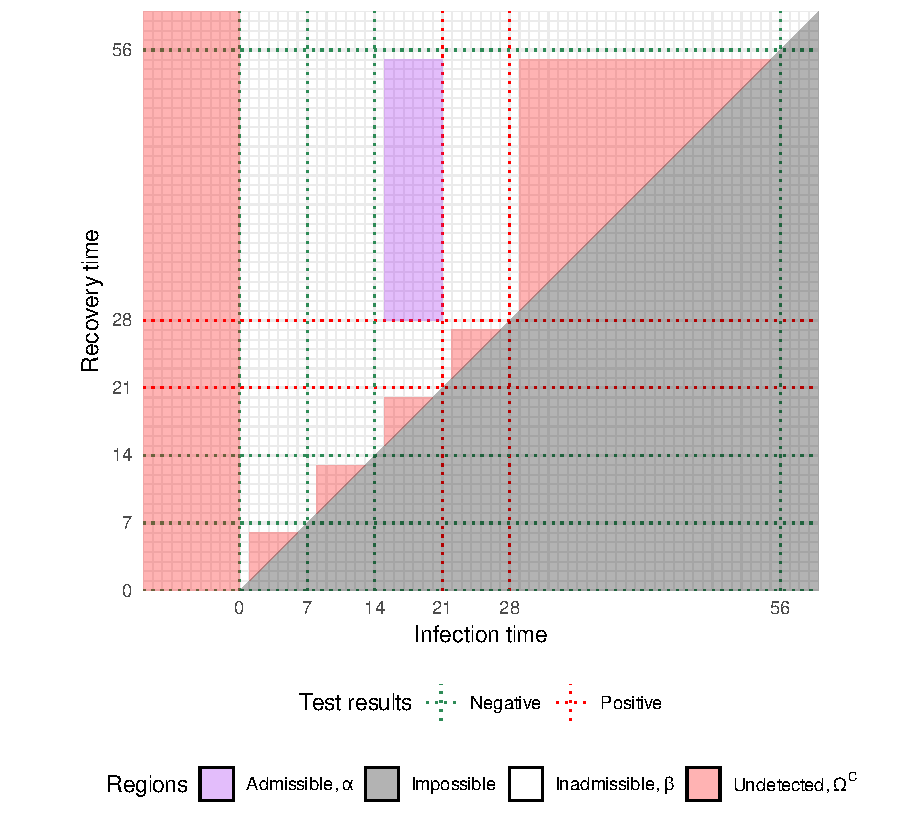
\includegraphics[width=\textwidth]{cis-perfect-testing/regions_diag}
\caption[Admissible, inadmissible, and undetected infections]{The regions (as defined in the main text) for an episode $i$ in an
individual whose first test was at time 0 and negative, with subsequent
negative tests at times 7, 14, and 56, and positive tests at times 21
and 28. Inadmissible region is unshaded. The black (impossible) region is because it does not make sense for recovery to occur prior to infection. \label{perf-test:fig:partitionSpace}}
\end{figure}

These three classes span all possible episodes and are mutually
exclusive, and hence the total number of episodes,
$n_i = n_{ia} + n_{iu} + n_{it}$, and
$p_{ia} + p_{iu} + p_{it} = 1$.

Episode $i$ and its ghosts independently belong to one of these
classes. Therefore, conditional on $n_i$, the number of episodes in
each class (that is, the counts $n_{ia}, n_{iu}, n_{it}$) are
distributed multinomially. Hence:
\begin{align}
&p(n_{ia} = 1, n_{iu} = 0, n_{it} = n_i - 1 \mid n_i, \theta) \\
&= \frac{n_i!}{n_{ia}! n_{iu}! (n_i- n_{ia} - n_{it})!} p_{ia}^{n_{ia}} p_{ua}^{n_{ia}} p_{it}^{n_i- n_{ia} - n_{it}} \\
&= \frac{n_i!}{(n_i-1)!} p_{ia} p_{it}^{n_i- 1} &\text{as $n_{ia} = 1$ and $n_{iu} = 0$}\\
&= n_i p_{ia} p_{it}^{n_i- 1}
\end{align}

The posterior we are interested in is
$p(\theta \mid n_{1a} = 1, n_{1u} = 0, \dots, n_{n_a,a} = 1, n_{n_a,u} = 0)$,
where $\theta$ are the parameters governing the survival distribution
and hence allow derivation of the $p$s.
\begin{align}
&p(\theta \mid n_{ia} = 1, n_{iu} = 0, \dots, n_{n_a,a} = 1, n_{n_a,u} = 0) \\
&\propto p(\theta) \prod_{i=1}^{n_a} p(n_{ia} = 1, n_{iu} = 0 \mid \theta) \\
&= p(\theta) \prod_{i=1}^{n_a} \sum_{n_i=1}^\infty p(n_{ia} = 1, n_{iu} = 0, n_{it} = n_i - 1 \mid \theta, n_i) p(n_i \mid \theta) \\
&= p(\theta) \prod_{i=1}^{n_a} \sum_{n_i=1}^\infty n_i p_{ia} p_{it}^{n_i- 1} p(n_i) \\
&= p(\theta) \prod_{i=1}^{n_a} p_{ia} \sum_{n_i=1}^\infty n_i p_{it}^{n_i- 1} p(n_i).\label{eqn:sum}
\end{align}


In the remainder of the section, expressions for $p_{ia}$,
$p_{it}$, and analytical solutions for the sum in \cref{eqn:sum} are derived in terms of the observed data, 
under different priors.

I derive an analytical solution to $\sum_{n_i=1}^\infty n_i p_{it}^{n_i- 1} p(n_i)$ under two different assumptions for $p(n_i)$.
First, we consider the improper prior $p(n_i) \propto 1/n_i$, this prior has several attractive properties.
Then, we consider a negative binomial distribution (which includes the geometric and Poisson distributions as a special and limiting case respectively).

The reference prior for $n_i$ is $p(n_i) \propto 1/n_i$~\autocite{heBayesiana}.
Under this prior,
$\sum_{n_i=1}^\infty n_i p_{it}^{n_i- 1} p(n_i) \propto \sum_{n_i=1}^\infty p_{it}^{n_i-1} = 1/(1-p_{it})$.
This likelihood is equal to the conditional likelihood used in the frequentist approaches previously mentioned.
It has been used elsewhere for Bayesian inference~\autocite{zhouUnified}, but the justification within a Bayesian paradigm has not been made explicitly.
%The prior $p(n_i) \propto 1/n_i$ means that the model coincides with the frequentist conditional likelihood approach, up to the priors on other parameters~\cites[section 4.2]{dempsterMaximum}{heiseyModelling}[section 8.7.5]{gelmanBayesian}.
% (\protect\hyperlink{ref-dempsterMaximum}{Dempster, Laird, and
% Rubin} (\protect\hyperlink{ref-dempsterMaximum}{1977}) section 4.2;
% \protect\hyperlink{ref-heiseyModelling}{Heisey and Nordheim}
% (\protect\hyperlink{ref-heiseyModelling}{1995});
% \protect\hyperlink{ref-gelmanBayesian}{Gelman et al.}
% (\protect\hyperlink{ref-gelmanBayesian}{2013}) section 8.7.5)

Now consider $N_i \dist \NegBin(\mu, r)$ using the
mean/dispersion parameterisation of the negative binomial. Equivalently:
\begin{align}
N_i \mid \lambda_i &\dist \Poi(\lambda_i) \\
\lambda_i &\dist \GamDist(a, b)
\end{align}
where $b = r / \mu$ and $a = r$.
Hence:
\begin{align}
\sum_{n_i=1}^\infty n_i p_{it}^{n_i- 1} p(n_i) 
&= \int \sum_{n_i=1}^\infty n_i p_{it}^{n_i- 1} p(n_i \mid \lambda_i) p(\lambda_i) d\lambda_i \\
&= \int \sum_{n_i=1}^\infty n_i p_{it}^{n_i- 1} \frac{\lambda_i^{n_i} e^{-\lambda_i}}{n_i!} p(\lambda_i) d\lambda_i \\
&= \int e^{-\lambda_i} \sum_{n_i=1}^\infty p_{it}^{n_i- 1} \frac{\lambda_i^{n_i-1}\lambda_i }{(n_i-1)!} p(\lambda_i) d\lambda_i \\
&= \int e^{-\lambda_i} \lambda_i p(\lambda_i) \sum_{n_t=0}^\infty p_{it}^{n_t} \frac{\lambda_i^{n_t} }{n_t!} d\lambda_i &n_t = n_i - 1 \\
&= \int e^{-\lambda_i} \lambda_i p(\lambda_i) e^{p_{it}\lambda_i} d\lambda_i &\text{Poisson pmf} \\
&= \int e^{\lambda_i (p_{it} - 1)} \lambda_i p(\lambda_i) d\lambda_i \\
&= \int e^{\lambda_i (p_{it} - 1)} \frac{b^a}{\Gamma(a)} \lambda_i^{a-1} e^{-b\lambda_i} \lambda_i d\lambda_i \\
&= \frac{\Gamma(a+1)b^a}{\Gamma(a) (b+1-p_{it})^{a+1}} \\ 
  &\; \times \int \frac{(b+1-p_{it})^{a+1}}{\Gamma(a+1)} \\
  &\; \lambda_i^{(a+1)-1} e^{-(b+1-p_{it})\lambda_i} d\lambda_i \\
&= \frac{\Gamma(a+1)b^a}{\Gamma(a) (b+1-p_{it})^{a+1}} &\text{as gamma pdf} \\
&\propto (b+1-p_{it})^{-(a+1)} \\
&= (r/\mu+1-p_{it})^{-(r+1)} \\
&\propto (r+\mu (1-p_{it}))^{-(r+1)}
\end{align}
Note that $r=0$ recovers the previous derivation (up to
proportionality).

The above allows us to sample from the posterior without needing to
sample the $n_i$s, which is much more efficient due to the previously-discussed dimensionality issue.
Furthermore, each $n_i$ is a discrete parameter, and hence
cannot be sampled with widely-used inference algorithms such as Stan's Hamiltonian Monte Carlo (HMC)\todo{ref}.

The posterior of $n_i$, while inconvenient to sample from and not of epidemiological interest directly, can be useful for diagnostic or model debugging purposes (for example, see\todo{ref where I use this in the next chapter}).
This posterior can be found by sampling from the full conditional.
Specifically, for each posterior sample of $\theta$, we sample one
draw from $n_i \mid \theta, y$ where $y$ represents all the data.

Due to the conditional independence of the $n_i$s, we find that:
\begin{align}
&p(n_i \mid \theta, n_{ia} = 1, n_{iu} = 0) \\
&\propto p(n_{ia} = 1, n_{iu} = 0, n_{it} = n_i - 1 \mid n_i, p_{iu}, p_{ia}, p_{it}) p(n_i) \\
&\propto n_i p_{it}^{n_i- 1} p(n_i)
\end{align}
With the prior, $p(n_i) \propto 1/n_i$ then this is a geometric
distribution with parameter $1 - p_{it}$. With a negative binomial
prior, we have:
\begin{align}
n_i p_{it}^{n_i- 1} p(n_i)
&\propto n_i p_{it}^{n_i- 1} \frac{\Gamma(r + n_i)}{n_i!} \left( \frac{\mu}{r+\mu} \right)^{n_i} \\
&\propto \frac{\Gamma((r + 1) + (n_i - 1))}{(n_i-1)!} \left( \frac{\mu p_{it}}{r+\mu} \right)^{n_i-1}
\end{align}
Therefore, by comparing this expression to the pmf of a negative binomial, we find that $n_i - 1$ is distributed negative binomial with size parameter $r+1$ and
probability parameter $\frac{r + \mu (1 - p_{it})}{r+\mu}$. The mean
of this distribution is
\begin{align}
\frac{(r+1)\mu p_{it}}{r+\mu(1-p_{it})}
\end{align}

Next, I derive $p_{ia}$ and $p_{it}$.

By definition, we have
\begin{align}
p_{ia} &= \prob((b, e) \in \alpha_i) \\
\alpha_i &= \{ (b, e) : l_i^{(b)} \leq b \leq r_i^{(b)} \wedge l_i^{(e)} \leq e \leq r_i^{(e)}\}.
\intertext{Hence:}
p_{ia}
&= \prob \left( l_i^{(b)} \leq B_i \leq r_i^{(b)}, l_i^{(e)} \leq E_i \leq r_i^{(e)} \right) \\
&= \prob \left( l_i^{(e)} \leq E_i \leq r_i^{(e)} \mid l_i^{(b)} \leq B_i \leq r_i^{(b)} \right) \prob \left( l_i^{(b)} \leq B_i \leq r_i^{(b)} \right) \\
&=\sum_{b = l_i^{(l)}}^{r_i^{(b)}} \prob \left( l_i^{(e)} \leq E_i \leq r_i^{(e)} \mid B_i = b \right) \prob \left(B_i = b \right) \\
&=\sum_{b = l_i^{(b)}}^{r_i^{(b)}} \prob \left( l_i^{(e)} - b + 1 \leq D_i \leq r_i^{(e)} - b + 1 \right) \prob \left(B_i = b \right) \\
&=\sum_{b = l_i^{(b)}}^{r_i^{(b)}} \left( S_\theta(l_i^{(e)} - b + 1) - S_\theta(r_i^{(e)} - b + 2) \right) \prob \left(B_i = b \right) \\
&\propto \sum_{b = l_i^{(b)}}^{r_i^{(b)}} \left( S_\theta(l_i^{(e)} - b + 1) - S_\theta(r_i^{(e)} - b + 2) \right)
\end{align}
under the assumption of uniform probability of infection time.

Next, we derive $p_{it} = \prob((b, e) \in \Omega^C_i)$, the probability
that episode $i$ was detected. A detected episode means that no test
was performed during the episode or there was no negative test prior to
the episode. Denote by $t_i$ the set of testing times for the
individual in which episode $i$ was observed, and define the time
until the next test on the individual after time $t'$ as:
\begin{align}
t^N_{it} &= \min \{ t' \in t_i : t' \geq t \} - t.
\intertext{Then:}
\Omega^C_i
&= \{ (b, e) : \nexists t \in t_i. b \leq t \leq e \vee b \leq \min(t_i) \} \\
&= \{ (b, e) : e - b < t^N_{ib} \vee b \leq \min(t_i) \}.
\intertext{Hence:}
1 - p_{it}
&= 1 - \prob(E_i - B_i < t_{iB_i}^N \vee B_i \leq \min(t_i)) \\
&= 1 - \prob(E_i - B_i < t_{iB_i}^N \wedge B_i > \min(t_i)) - \prob(B_i \leq \min(t_i)) \\
&= 1 - \sum_{b=\min(t_i) + 1}^T \prob(E_i - b + 1 < t_{ib}^N \mid B_i = b) \prob(B_i = b) \\
  &\; - \sum_{t=1}^{\min(t_i)} \prob(B_i = b)\\
&= 1 - \frac{1}{T} \sum_{b=\min(t_i)+1}^T (1 - S_\theta(t_{ib}^N + 1)) - \frac{\min(t_i)}{T} \\
&= 1 - \frac{T-\min(t_i)}{T} + \frac{1}{T} \sum_{b=\min(t_i)+1}^T S_\theta(t_{ib}^N + 1)) - \frac{\min(t_i)}{T} \\
&= \frac{1}{T} \sum_{b=\min(t_i)+1}^T S_\theta(t_{ib}^N + 1)
\end{align}

\subsection{Full posterior}\label{perf-test:sec:full-posterior}

Under the prior $p(n_i) \propto 1/n_i$:
\begin{align}
&p(\theta \mid n_{ia} = 1, n_{iu} = 0, \dots, n_{n_a,a} = 1, n_{n_a,u} = 0) \\
&\propto p(\theta) \prod_{i=1}^{n_a} p_{ia} \sum_{n_i=1}^\infty n_i p_{it}^{n_i- 1} p(n_i) \\
&= p(\theta) \prod_{i=1}^{n_a} \frac{p_{ia}}{1-p_{it}} \\
&\propto p(\theta) \prod_{i=1}^{n_a} \frac{\sum_{b = l_i^{(b)}}^{r_i^{(b)}} \left( S_\theta(r_i^{(e)} - b - 1) - S_\theta(l_i^{(e)} - b - 1) \right)}{\sum_{b=\min(t_i)}^T S_\theta(t_{ib}^N + 1)} \\
\end{align}

Under the prior $N_i \dist \text{NegBinom}(\mu, r)$:
\begin{align}
&p(\theta \mid n_{ia} = 1, n_{iu} = 0, \dots, n_{n_a,a} = 1, n_{n_a,u} = 0) \\
&\propto p(\theta) \prod_{i=1}^{n_a} p_{ia} \sum_{n_i=1}^\infty n_i p_{it}^{n_i- 1} p(n_i) \\
&= p(\theta) \prod_{i=1}^{n_a} \frac{p_{ia}}{(r+\mu (1-p_{it}))^{(r+1)}} \\
&= p(\theta) \prod_{i=1}^{n_a} \frac{\sum_{b=l_i^{(b)}}^{r_i^{(b)}} \left( S_\theta(r_i^{(e)} - b - 1) - S_\theta(l_i^{(e)} - b - 1) \right)}{\left( r+\mu/T \left( \sum_{b=\min(t_i)}^T S_\theta(t_{ib}^N + 1) \right) \right)^{(r+1)}} \\
\end{align}

\section{Parameterisation and priors for the survival function} \label{perf-test:sec:parameters-priors}

The form of $S_\theta(t)$ is yet to be specified.
As frequently observed in the literature~\autocite[e.g.:][]{heBayesian}, it is more convenient to operate with the hazard than the survival or probability mass function directly.
This is because the mass function must sum to one and the survival must be monotonically decreasing, while there are no constraints across multiple hazards.
The only constraint on the hazard is to be in the interval $[0, 1]$, since they are probabilities.

In this section, I consider the various parameterisation of the survival function that are available.
This has implications for the choice of prior it is not possible to be vague on all sensible parameterisations.
Informative priors might also be attractive, and allow the incorporation of the estimates from \cref{E-ATACCC}.

The hazard is convenient to use because it is unconstrained except in the interval [0, 1].
The [0, 1] interval is easily be mapped to the unconstrained reals using a logit transformation (where $\logit(x) = \log(x/(1-x))$).
Conversely, the survival function, $S_\theta(t)$, needs to be monotonically decreasing.
Therefore, there is a constraint on $S_\theta(t)$ which depends on $S_\theta(t-1)$.
This complicates the inference process and cannot be removed through a simple transformation.

The rest of this section considers appropriate priors for the hazard in this context.

\subsection{Independent priors} \label{perf-test:sec:independent-priors}
Take the standard assumption of independent priors on each parameter.
Each hazard, $\lambda_t$, is a (conditional) probability, and hence a Beta distribution is a natural choice.

Uninformative Beta priors on the hazard are problematic in this context.
An uninformative prior would be of the form $\lambda_t \dist \Beta(\alpha, \alpha)$.
Commonly, $\alpha$ is chosen to be $0.5$ (Jeffreys' Prior) or $1$ (a uniform prior).
Even though these priors are uninformative on the hazard, they become highly informative on the survival. 
Specifically, they tend to favour shorter survival times (see \cref{perf-test:fig:flat-prior}).
An intuitive explanation of this can be drawn from the fact that these types of priors have an expected value of 0.5.
The expected survival time, $\E \left( \prod_{i=1}^{t-1} (1-\lambda_t) \right)$, is therefore equal to $0.5^{t-1}$, a quantity that declines rapidly.
This prior expresses extreme scepticism in estimates from previous studies, such as \cref{E-ATACCC} and the meta-analysis of \textcite{cevikShedding}.
\begin{figure}
  \centering 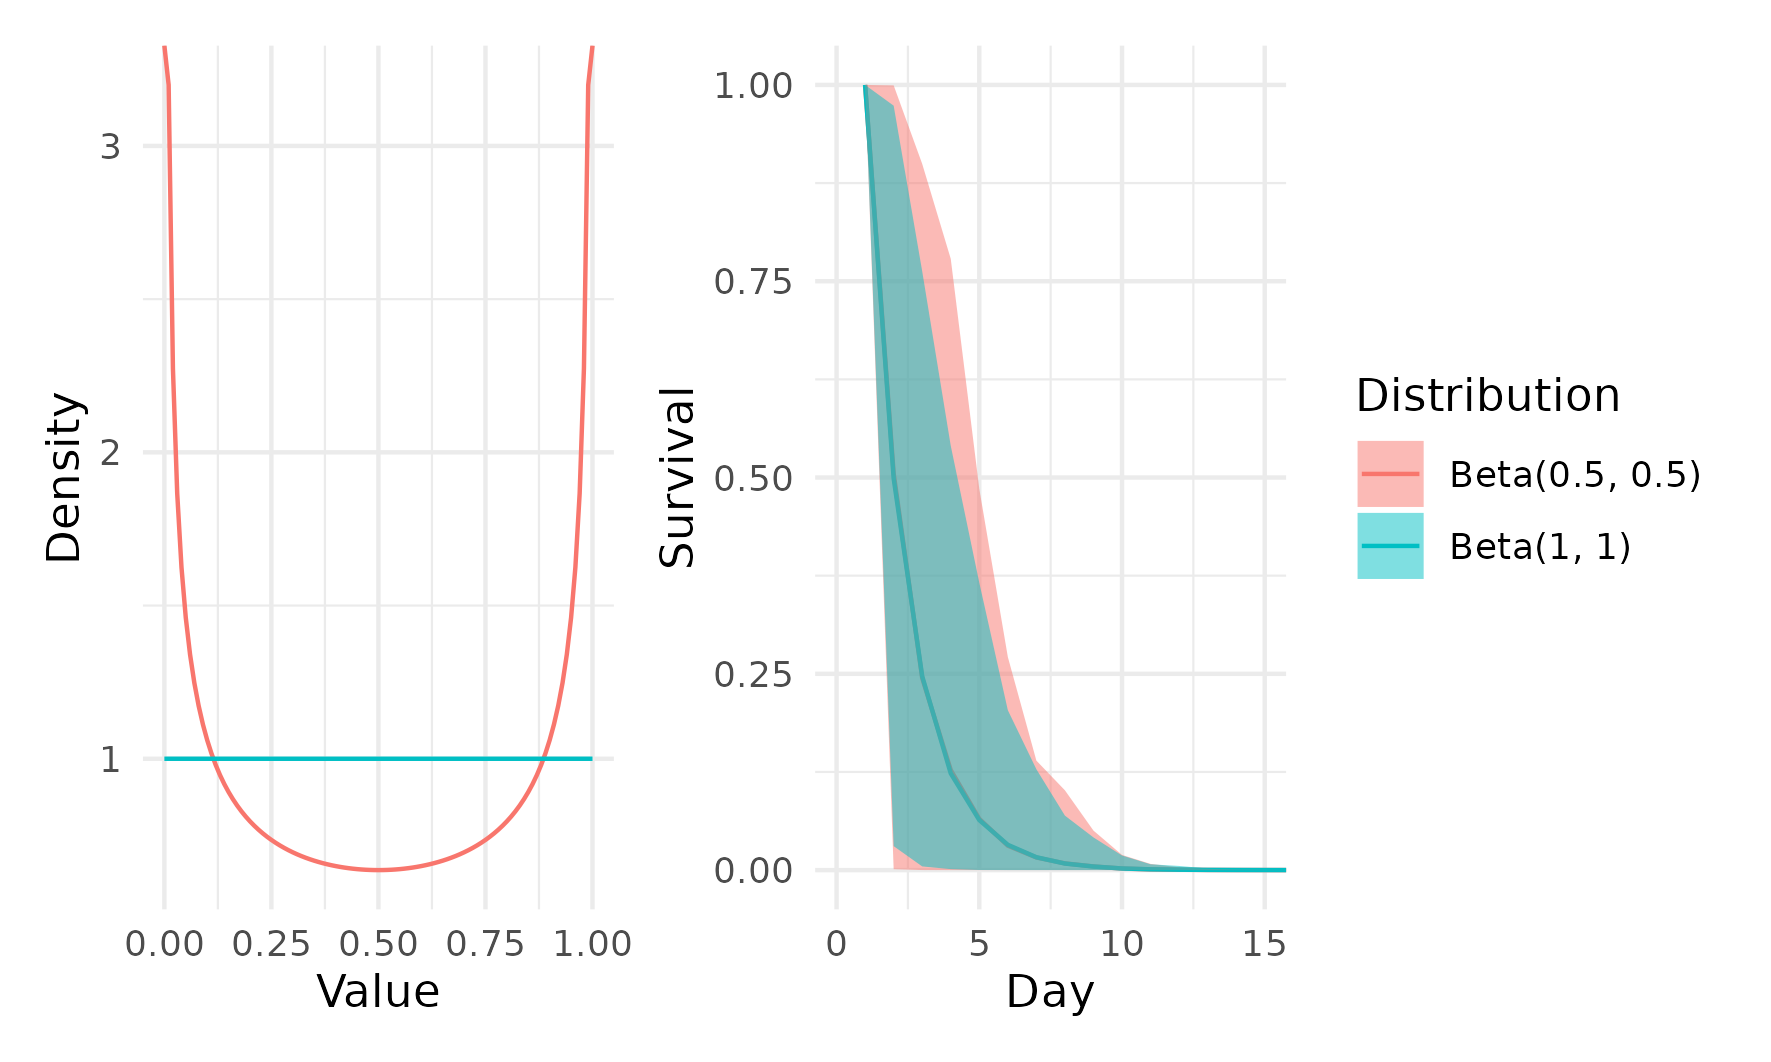
\includegraphics{cis-perfect-testing/flat-prior}
  \caption[Uninformative priors for the hazard]{The density of Beta(1, 1) flat prior and Beta(0.5, 0.5) uninformative priors (left) with the prior predictive survival time (right). The implied prior on the survival time is very short when using either prior on the hazard at each time. \label{perf-test:fig:flat-prior}}
\end{figure}

Instead, I propose a weakly informative prior Beta(0.1, 1.9), which has mean 0.05 and minimal information.
The amount of information in a Beta distribution is related to the sum of its parameters.
Here, the sum equals 2, the same as the flat prior case.
The central 95\% probability mass of Beta(0.1, 1.9) is 0.00--0.47.
The central estimate, of 0.05, is in line with previous estimates that the median duration is in the range 15--20 days~\autocite{cevikShedding}.
This prior gives a very vague prior predictive distribution on the survival time (see \cref{perf-test:fig:vague-prior}).
\begin{figure}
  \centering 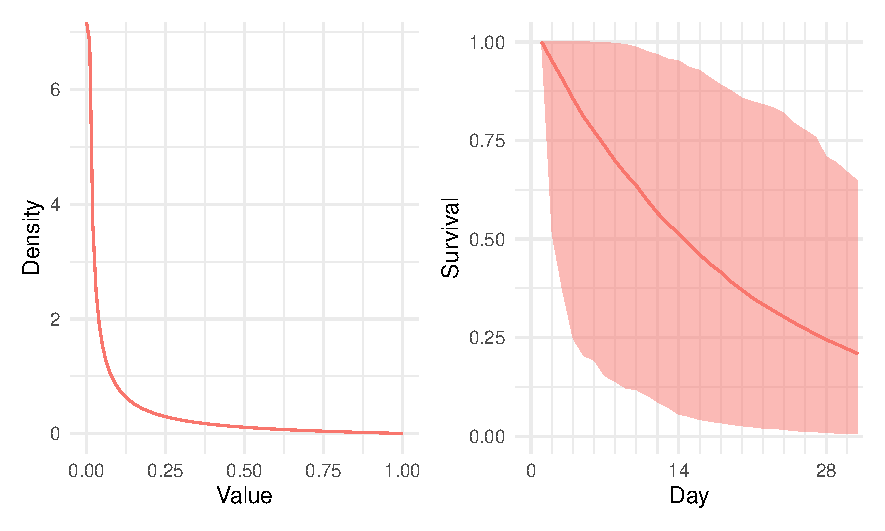
\includegraphics{cis-perfect-testing/vague-prior}
  \caption[Weakly informative priors for the hazard]{The density of Beta(0.1, 1.9) vague prior (left) and the prior predictive survival time (right). The prior predictive survival time is very vague using a Beta(0.1, 1.9) prior. Note the different x-axis to \cref{perf-test:fig:flat-prior}. \label{perf-test:fig:vague-prior}}
\end{figure}


\subsection{Smoothing priors}

Smoothing priors encode the biological consideration that the hazard should not vary significantly from day-to-day.
It is the Bayesian equivalent of a penalised likelihood, used frequently in the non-parametric frequentist setting (\eg: \autocite{bacchettiNonparametric}).
Many possible forms of smoothing priors exist, including splines, Gaussian Processes, and random walks.
I use a second-order random walk because it is simple and can produce sensible prior predictive distributions.

A second-order random walk prior encodes that the hazard should be linearly changing with some random changes at each time step.
Specifically, the difference between $\lambda_t$ to $\lambda_{t+1}$ is the difference between $\lambda_{t-1}$ and $\lambda_t$ plus some Gaussian-distributed noise.
Formally:
\begin{align}
  \logit\lambda_{t+1}
  &= \logit\lambda_t + (\logit\lambda_t - \logit\lambda_{t-1}) + \sigma \epsilon_t &\text{for $t \geq 2$} \\
  &= 2\logit\lambda_t - \logit\lambda_{t-1} + \sigma \epsilon_t \\
  \epsilon_t &\dist N(0, 1) &\text{for $t \geq 2$}  \\
  \logit\lambda_2 &= \logit\lambda_1 + \epsilon_1 \\\
  \epsilon_1 &\dist N(\mu_{\epsilon_1}, \sigma_{\epsilon_1}^2) \\
  \logit \lambda_1 &\dist N(\mu_{\lambda_1}, \sigma_{\lambda_1}^2) \\
  \sigma &\dist \Exponential(1/\mu_\sigma).
\end{align}
The hyperparmeters $\mu_{\lambda_1}$ and $\sigma_{\lambda_1}$ specify the prior on the hazard at time 1; $\mu_{\epsilon_1}$ and $\sigma_{\epsilon_1}$ the prior on the initial gradient; and $\mu_\sigma$ the smoothness of the random walk.
I use $\mu_{\lambda_1} = -17.5$, $\sigma_{\lambda_1} = 6$, $\mu_\epsilon = 1.09$, $\sigma_\epsilon = 0.03$, and $\mu_\epsilon = 0.1$ based on the analysis in \cref{E-ATACCC}.

\subsection{Model combination priors} \label{perf-test:sec:informative-priors}

I propose combining the information from the CIS data with \cref{E-ATACCC}'s analysis by using \cref{E-ATACCC}'s analysis as a prior for the CIS analysis.
This is desirable because the ATACCC study frequently samples individuals early in the infection.
Therefore, that analysis's estimate of the survival distribution in the early infection period should be reliable.
In the later infection period, the ATACCC study has fewer observations and hence the estimates are less reliable; CIS can then inform the posterior in this region.

In the combination methodology, two aspects need to be considered.
Firstly, the model structure from \cref{E-ATACCC} leads to positive correlation in the posterior estimates of the hazard, which should be propagated into this analysis.
That is, the prior used in this analysis cannot be independent across the hazards.
Secondly, the uncertainty in the estimates from \cref{E-ATACCC} should be increased for this analysis.
The additional uncertainty is because the \cref{E-ATACCC} analysis extrapolates beyond the data using strong model assumptions (see \todo{reference discussion on extrapolation in ATACCC chapter}).
Furthermore, there are differences in the study design and laboratories used between the two studies (see \cref{E-intro:sec:studies}) which may mean that results do not generalise between the studies.
I form the prior for the combination in two steps.

I first approximate the \cref{E-ATACCC} posterior estimate of the hazard as a multivariate normal on the logit scale.
This can be viewed as an approximation of Markov melding~\autocite{goudieJoining}.
Using a multivariate normal, as opposed to multiple univariate distribution, ensures that the correlation between the hazards is preserved.
The logit transformation maps from the $[0, 1]$ interval to the full real line.
To estimate the parameters of the multivariate normal, I use the method of moments.
The approximation is very good (see \cref{perf-test:fig:approximate-ATACCC-hazard} and \cref{perf-test:fig:approximate-ATACCC-survival}).
\begin{figure}
  \thisfloatpagestyle{empty}
  \vspace{-2.5cm}
  \makebox[\textwidth][c]{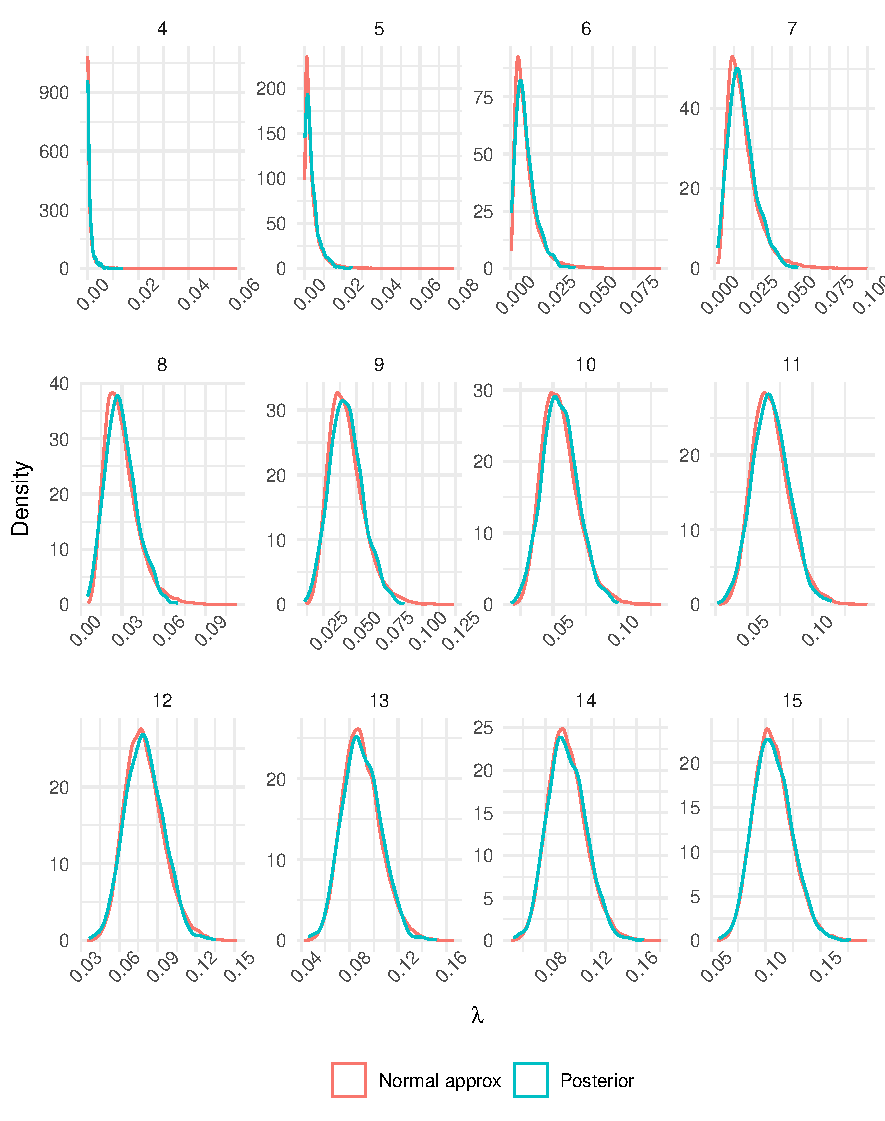
\includegraphics[width=.9\paperwidth]{cis-perfect-testing/ataccc-approximation-hazard}}
  \caption[Approximating the ATACCC posterior hazard as a logit-normal]{Comparison of the posterior estimate of the hazard from \cref{E-ATACCC} and its approximation with a logit-normal distribution (kernal density estimate smoothed) for the first 15 hazards. \label{perf-test:fig:approximate-ATACCC-hazard}}
\end{figure}
\begin{figure}
  \centering 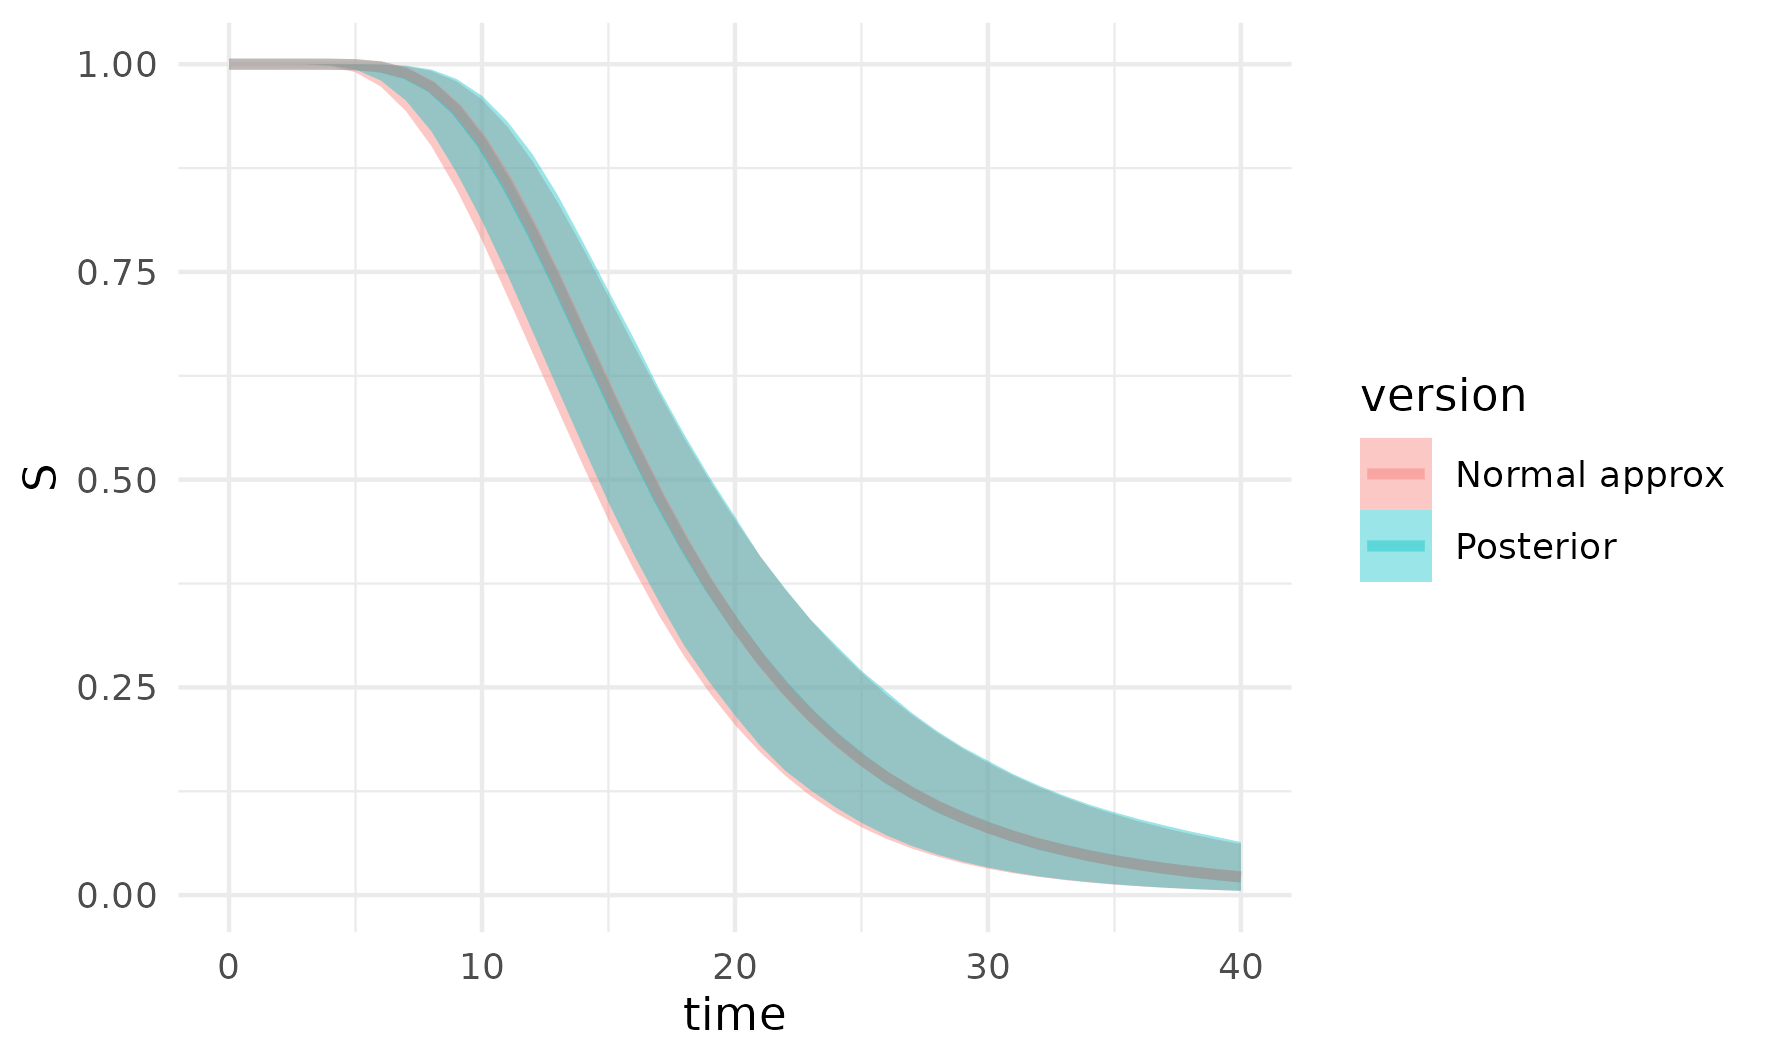
\includegraphics{cis-perfect-testing/ataccc-approximation-survival}
  \caption[Approximating the ATACCC posterior survival as a logit-normal]{Comparison of the posterior estimate of the survival from \cref{E-ATACCC} and its approximation with a logit-normal distribution (median and central 95\% interval). The survival is a function of all the hazards up until that point, therefore the correlation between the hazards must be well-approximated to have these agree. \label{perf-test:fig:approximate-ATACCC-survival}}
\end{figure}

Having approximated the estimate as a multivariate normal, I add additional uncertainty using a discrete Beta process.
The discrete Beta process prior generalises the form of prior used in \cref{perf-test:sec:independent-priors} by allowing the central estimate of the hazard to vary over time~\autocites{ibrahimBayesian}{sunStatisticala}.
It is:
\begin{align}
  \lambda_t &\sim \text{Beta}(\alpha_t, \beta_t) &t = 1, 2, \dots \\
  \alpha_t &= c_t h_t + \alpha_0 \\
  \beta_t &= c_t (1 - h_t) + \beta_0
\end{align}
where $k_t$, $\alpha_0$, and $\beta_0$ are hyperparameters; and $h_t$ is a point estimate of the hazard at time $t$ from ATACCC.
An intuition for what this distribution represents can be gained by considering the conjugate model for $\lambda_t$ with a beta prior and a binomial likelihood.
If $\lambda_t$ is given the prior distribution $\text{Beta}(\alpha_0, \beta_0)$, and we then have $k_t$ observations with $k_t h_t$ successes, then the posterior distribution for $\lambda_t$ is $\text{Beta}(\alpha_t, \beta_t)$ (as defined above).

\section{Simulation study} \label{perf-test:sec:simulation-study}

\subsection{Setup}

I simulate a dataset of detected episodes that has the same characteristics as that in the CIS by the following procedure.
\begin{enumerate}
    \item Extract the test schedules for each individual who had at least one test during the period of interest.
    \item Draw an episode start time, $b_i$ for each individual uniformly at random between 2nd July 2020 (100 days before the period where a detected episode would be included) and 6th December 2020 (the end of this period).
    \item Draw a duration of episode for each individual, $d_i$, based on the distribution described below. Then calculate the end of their infection episode, $e_i = b_i + d_i - 1$.
    \item Simulate the test results based on the test schedule, $b_i$, and $e_i$. Tests between $b_i$ and $e_i$ (inclusive) are positive, all other tests are negative.
    \item Discard episodes where there are no positive tests (\ie undetected episodes) and then apply the same inclusions/exclusions as in \cref{perf-test:sec:problem}.
    \item Of these remaining episodes, sample 4,800 to match the sample size of the true dataset. This is needed because in step 2 the entire cohort was infected, while in the real study only a (unknown) portion is infected.
    \item For this final set of episodes, calculate $(l_i^{(b)}, r_i^{b}, l_i^{(e)}, r_i^{(e)})$ by taking the day after the last negative prior to any positives, the first positive, the last positive, and the day before the negative following the last positive respectively.
\end{enumerate}

To generate the durations, an assumption is required for the distribution of the duration of positivity.
I base this assumption on the estimate from \cref{E-ATACCC} with an inflated tail to represent what is seen within CIS.
The tail is modified based on an unpublished analysis of CIS data by Sarah Walker (described below).
Sarah uses survival analysis to estimate the duration from CIS data.
The initiating event is assumed known as the time the episode was detected.
The final event is assumed interval-censored between the time of the final positive test and the subsequent negative test, or right-censored if a negative test has not yet been observed.
A flexible, spline-based form is assumed for the baseline survival function~\autocite{roystonSTPM,roystonFlexible} with covariates introduced via proportional odds.
By not accounting for either the undetected infections or the interval censoring of the initiating event, this analysis has competing biases which makes them hard to interpret~\autocite{cisMethodsONS}.

% \todo[inline]{The following seems important to justify why we can't just use these estimates but is also basically an aside}
% We know of two biases introduced from this analysis.
% \enquote{There is a bias in estimating the clearance distribution because the analysis used to estimate how long a person stays positive only starts from their first positive test.
% Since (most) people will have become positive on an earlier day, this will bias the clearance curves downwards (making the estimates too short).
% However, there is another bias due to the survey missing positive episodes entirely if they are short.
% This means that our dataset has fewer short positive episodes than in the population as a whole, and that the sample used to run the survival analysis is biased towards people with longer positive episodes.
% This will bias the clearance curves upwards (making the estimates too long).}~\autocite{cisMethodsONS}.

To form the duration distribution used in the simulation, we combine the two estimates.
The first 30 days of the distribution is proportional to the ATACCC estimate, with the rest proportional to this CIS-based estimates.
% The CIS-based estimates are shifted 3 days in order to make this smooth; this counteracts the above bias of missing the start of the infection (for times above 30 days, the other bias, missing short infections, is negligible). ERR... I'M NOT DOING THIS ANYMORE OH NO!!
Denote by $f_A(t)$ the distribution function estimated from ATACCC and $f_C(t)$ that from these CIS-based estimates.
Then define:
$$
f_S'(t) = \begin{cases}
	f_A(t) &t \leq 30 \\
	f_C(t) &t > 30
\end{cases}
$$
Then the distribution used in the simulation is the normalised version of this: $f_S(t) = f'_S(t)/\sum_i f_S'(i)$.
These curves and the combined curve are compared in \cref{perf-test:fig:duration-dist}.
Individual $i$'s duration of positivity, $D_i$, is then an independent draw from this distribution.
\begin{figure}
  \centering 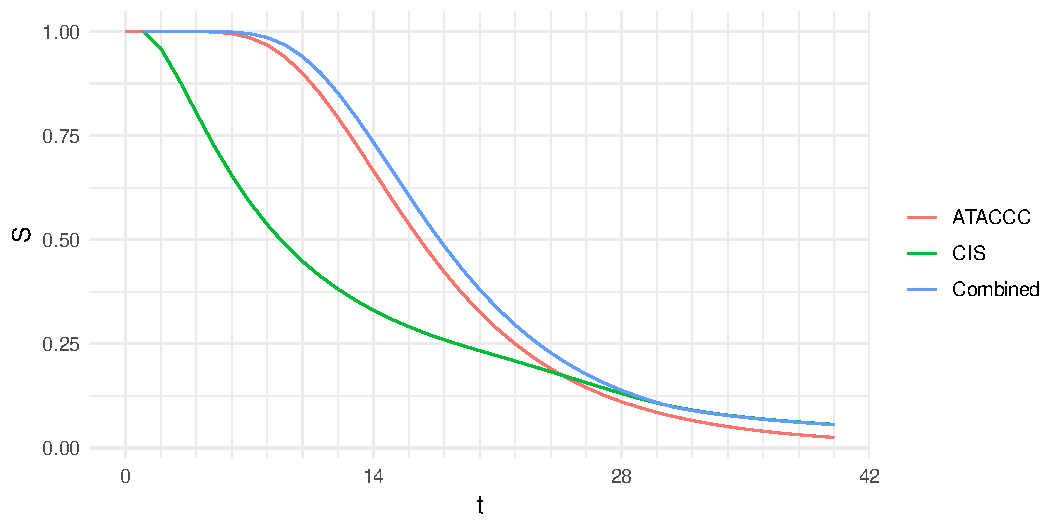
\includegraphics{cis-perfect-testing/input-duration-dists}
  \caption[Comparison of duration distributions]{Comparison of the duration distribution used for the simulation. ATACCC is the posterior mean from \cref{E-ATACCC}'s analysis, CIS is Sarah Walker's analysis, and Combined is the combination of these used for the simulation. See main text for details of each analysis. \label{perf-test:fig:duration-dist}}
\end{figure}

\subsection{Implementation}

Simulation was performed in R~4.2.0~\autocite{R4-2-0} using tidyverse~2.0.0~\autocite{tidyverse} and targets~1.1.3~\autocite{targetsPackage}.

Inference was implemented in Stan via RStan~2.21.8~\autocite{rstan2-21-8} using default settings.
Convergence was assessed using Rhat and ESS as described in \cref{E-ATACCC:sec:convergence}, and all runs checked for divergent transitions.

The prior on the total number of infections was TBD\todo{fill in once decided on total vs individual model}.

A framework for performing CIS-like simulations is available at \url{https://github.com/joshuablake/cisSimulation}.
A framework for fitting the class of models described here and in \cref{E-imperf-test} is available at \url{https://github.com/joshuablake/cisDurationModel}.
Code utilising these frameworks to perform the analysis described in this chapter is available at \url{https://github.com/joshuablake/cisRuns}.

\subsection{Results}

All analyses converged satisfactorily\todo{put numbers once confirmed exact analyses to use}.
Repeating simulations showed very little variation in the results, due to the large sample size in CIS; therefore, only results from a single simulation are shown.

The true value of the survival function is very well recovered with little difference between priors (see \cref{perf-test:fig:survival-results}).

The independent prior has the fewest assumptions and least prior information.
Therefore, it leads to posterior estimates that are most uncertain.

The second-order random walk is the only prior that smooths the hazard throughout the entire infection.
This leads to a near-constant hazard, and hence exponential-like survival, in areas where there is little information (long infections).

\begin{figure}
  \centering 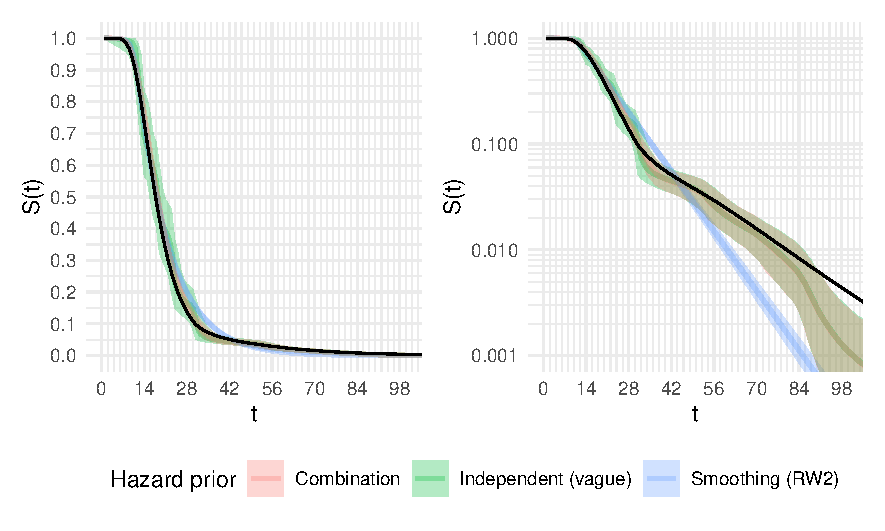
\includegraphics{cis-perfect-testing/survival-results}
  \caption[Comparison of survival function estimates under different priors]{Comparison of the posterior estimate of the survival distribution (pointwise median and 95\% CrI) when using different priors on the hazard. Results using each of the three different priors discussed in \cref{perf-test:sec:parameters-priors} are shown. \label{perf-test:fig:survival-results}}
\end{figure}

\begin{figure}
  \centering 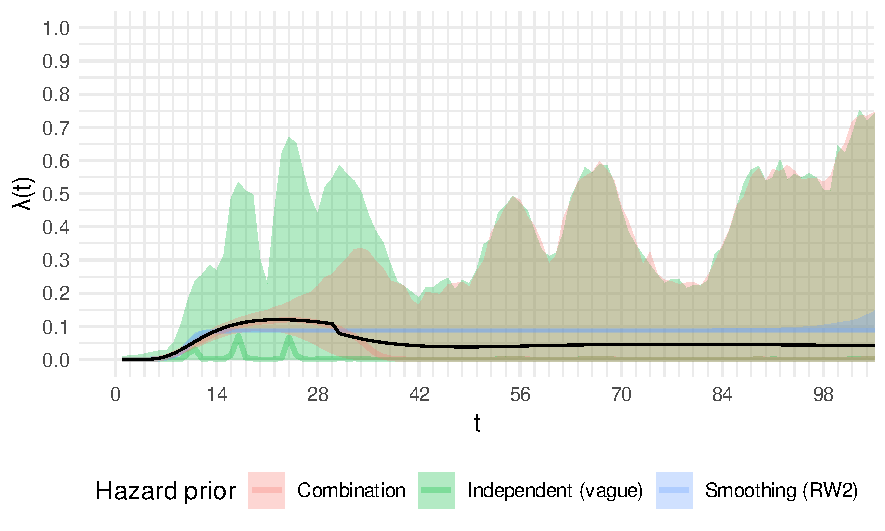
\includegraphics{cis-perfect-testing/hazard-results}
  \caption[Comparison of hazard estimates under different priors]{Comparison of the posterior estimate of the hazard (pointwise median and 95\% CrI) when using different priors on the hazard. Results using each of the three different priors discussed in \cref{perf-test:sec:parameters-priors} are shown. \label{perf-test:fig:hazard-results}}
\end{figure}

\section{Discussion} \label{perf-test:sec:discussion}

This chapter shows that the model I propose can recover the true survival function well, is not sensitive to the prior used for the survival distribution, nor requires information on the number of infections that were undetected.
However, the problem becomes substantially harder if false negatives are present, as we shall see in the next chapter.
Unfortunately, false negatives do occur in the CIS data.

Various extensions could be worth exploring.
Most importantly, covariates (\eg age, immunity from vaccination and/or previous infection, or variant) could be included.
Immunity in particular affects the duration substantially, although age and variant may also make a contribution~\autocites{hakkiOnset}{russellWithinhost}.
Covariates can be included with a variety of model, the simplest being a proportional hazards model.

The form of priors used for the survival function could also be extended.
In particular, the form of smoothing chosen here is very simple and could be replaced with a more flexible model, such as a Gaussian Process for additional flexibility and smoothing and different time-scales~\autocite{saulGaussian}.

The prior would likely be more important if the number of detected infections was smaller.
Therefore, exploring its impact would be important for designing future surveys.
A particular application would be estimation in the early stages of an epidemic of a novel pathogen.
Here, little would be known about the pathogen, but gathering information with robust estimates of uncertainty is important to inform the response.

I have assumed constant and independent incidence (a priori).
In this case, a sensitivity analysis (not shown) showed minimal impact on survival estimates.
Furthermore, I chose a period where the incidence was approximately constant.
However, this assumption could be important in other contexts, especially if the incidence is changing rapidly.
The assumption of constant incidence can lead to biased estimates~\autocite{degruttolaAnalysis}.

\section{Conclusion} \label{perf-test:sec:conclusion}
This chapter has shown the feasibility of estimating the survival function from a study with a CIS-like testing schedule.
While the infrequent testing schedule is not ideal, appropriate modelling can recover the true survival function well.

\ifSubfilesClassLoaded{
  \appendix
  \subfile{appendix-cis-perfect-testing}
  \listoftodos
}{}
\end{document}